\documentclass{beamer}
\mode<presentation>
\usecolortheme{crane}

% \setbeamercovered{again covered={\opaqueness<1->{70}}}

\hfuzz=20pt

\setbeamertemplate{navigation symbols}{
\usebeamerfont{footline}
\usebeamercolor[fg]{footline}
\hspace{1em}
\insertframenumber/\inserttotalframenumber
}

\setbeamertemplate{caption}{\raggedright\insertcaption\par}


\usepackage{xifthen}
\usepackage{anyfontsize}
\usepackage{fontawesome}
\usepackage{filecontents}
\usepackage{bm}
\usepackage{tikz}
\usepackage{pgfplots}

\pgfplotsset{compat=1.15}
\usetikzlibrary{
	positioning
	,plotmarks
	,shapes.callouts	
    ,intersections	
	,decorations.pathreplacing
	,patterns
}
% Commands
\newcommand{\edge}[3][]{
	\draw[#1] (#2) edge (#3);
}

\newcommand{\edgeWithLabel}[4][]{
	\draw[#1] (#2) edge node[edge label]{#3} (#4);
}

\newcommand{\twocolors}[1]{
	\fill[fill=orange] (#1.west) -- (#1.east) arc(0:180:7.5pt);
	\fill[fill=blue] (#1.west) -- (#1.east) arc(0:-180:7.5pt);
	\node at(#1){};
}

% Animation
\tikzset{
	on/.code args={<#1>#2}{
  		\only<#1>{\pgfkeysalso{#2}}
	},
	alt/.code args={<#1>#2#3}{
  		\alt<#1>{\pgfkeysalso{#2}}{\pgfkeysalso{#3}}
	},
	hide/.style={
		opacity=0
	},
	show/.style={
		opacity=1
	},
	hide nodes/.style={
		every node/.append style={hide}
	},
	hide nodes text/.style={
		every node/.append style={text=white}
	},
	show nodes/.style={
		every node/.append style={show}
	},
	show nodes text/.style={
		every node/.append style={text=black}
	},
	blur/.style={
		opacity=0.2
		,text=white
	}
}

% Note
\tikzset{
	note/.style={
		rectangle callout
		,fill=#1
		,thin
		,inner sep=1mm
	}
	,noteorange/.style={note=orange!50}
}


% Label
\tikzset{
	label/.style={
		rectangle,	
		draw=none,
		fill=white,
		% font=\tiny,
		% font=\scriptsize,
		font=\footnotesize,
		inner sep=2pt,
		minimum height=0,
		minimum width=0,
	},
	edge label/.style={
		label,
		midway,
		sloped,
	},
	edge label below/.style={edge label, below=1mm},
	edge label above/.style={edge label, above=1mm},
}


% DEFAULTS
\tikzset{default node/.style={
	draw, 
	circle,
	inner sep=0mm,
	minimum size=5mm,
	font=\small,
}}

\tikzset{
	>=latex
	,every node/.style={default node}
	,every picture/.append style={very thick, black!70}
}
\newtheorem{observation}{Observation}

\DeclareMathOperator*{\argmin}{arg\,min}
\DeclareMathOperator*{\argmax}{arg\,max}

\def\R{\mathbb{R}}
\def\N{\mathbb{N}}

\def\1star{{\color{orange} \faStar}}
\def\2star{{\color{orange} \faStar\faStar}}
\def\3star{{\color{orange} \faStar\faStar\faStar}}

\def\pointer{callout absolute pointer}

\title{
Approximation Algorithms 
\\
for the
\\
Maximum Carpool Matching Problem
\\
and 
\\
Submodular Maximization
}
\author[shortname]{
    \textbf{Gilad Kutiel}
}
\date{2019}


\begin{document}

% \begin{frame}
\titlepage
\end{frame}

% \begin{frame}{Maximum Star Forest (SF)}
\begin{center}
\begin{tikzpicture}[-, thick,x=11mm]

\foreach[count=\i] \x \y in {
	0/0
	,2/1
	,1/2
	,3/4
	,4/-3
	,4/2
	,2/-2
	,3/-1
	,4/0
	,5/-2
	,6/1
	,5/3
	,7/-1
	,6/-3
	,7/2
	,9/0
	,8/3
	,8/-2
}{
	\node(\i) at(\x,\y){};
}

\foreach \u \v in {
	1/3,1/2,1/8,1/7%
	,6/4,6/9,6/10,6/11,6/15,6/12%
	,14/5%
	,16/13,16/17,16/18%
}{
	\draw (\u) -- (\v);
}

\foreach \u \v in {
	2/3,2/8,2/9,2/4,2/6%
	,3/4%
	,4/12,4/17%
	,5/7,5/8,5/9,5/10%
	,7/8%
	,8/9%
	,9/10%
	,10/11,10/11,10/13,10/14,10/18%
	,11/13,11/15,11/16%
	,12/15,12/17%
	,13/18%
	,15/16,15/17%
	,18/14%
}{
	\draw[on=<2>{blur}] (\u) -- (\v);
}


\end{tikzpicture}
\end{center}
\end{frame}
% \begin{frame}{Maximum Carpool Matching}
\begin{center}
    \begin{tikzpicture}[x=2cm,y=1.5cm, ->]
        \foreach[count=\i] \a \r \c \p in{
            0/1/\faCar/\faFemale
            ,10/2/\faBicycle/\faMale
            ,30/3/\faCab/\faChild
            ,160/1/\faMotorcycle/\faFemale
            ,230/1/\faTruck/\faMale
            ,-40/2/\faCar/\faFemale
            ,100/1/\faBicycle/\faMale
            ,80/2/\faCab/\faFemale
            ,-10/3/\faMotorcycle/\faBlind
            ,20/4/\faTruck/\faMale
            ,-100/2/\faCar/\faFemale
            ,-30/4/\faBicycle/\faMale
        }{
            \node[draw=none, inner sep=1mm](\i) at(\a:\r) {\c~\p};
        }
    
        \pause
        \foreach \u \w \v in{
            1/2/5%
            ,8/5/7%
            ,9/6/6%
            ,10/5/2%
            ,11/4/5%
            ,12/3/6%
        }{
            \edgeWithLabel[bend left, on=<3>{orange}]{\u}{\w}{\v}
        }
    
        \foreach \u \w \v in{
            1/2/2,1/2/4,1/3/6,1/2/7%
            ,2/4/3%
            ,3/6/10%
            ,4/7/7%
            ,5/3/4,5/9/11%
            ,6/1/9,6/5/11%
            ,7/4/1,7/3/8%
            ,8/5/3%
        }{
            \edgeWithLabel[bend left, on=<3>{blur}]{\u}{\w}{\v}
        }
    
    \end{tikzpicture}
\end{center}
\end{frame}
% \begin{frame}{Maximum Carpool Matching cont.}
\begin{center}
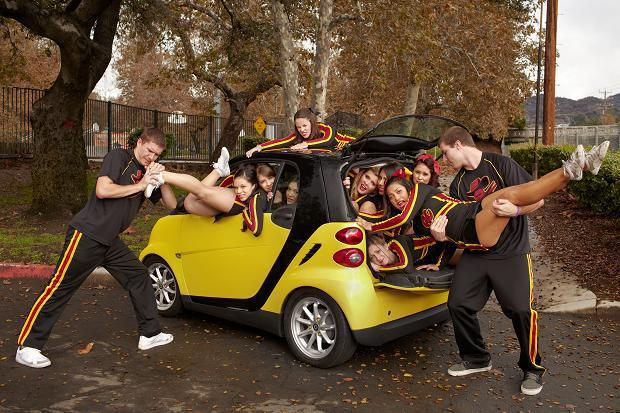
\includegraphics[scale=.5]{capacity}
\end{center}
\end{frame}
% \begin{frame}{Many Variants}
\def\pointer{callout absolute pointer}
\vfill
\begin{center}
\begin{tikzpicture}[every node/.style={note=orange!50}, x=16mm]
\draw (0,0) -- (6,0);
\node[\pointer={(0,0)}] at(0, 1) {SF};
\node[\pointer={(1,0)}] at(1, -1) {Node weighted SF};
\node[\pointer={(2,0)}] at(2, 1) {Edge weighted SF};
\node[\pointer={(3,0)}] at(3, -2) {Unweighted, O(1) capacity CM};
\node[\pointer={(4,0)}] at(4, 2) {Unweighted CM};
\node[\pointer={(5,0)}] at(5, -1) {CM};
\node[\pointer={(6,0)}] at(6, 1) {Group CM};
\end{tikzpicture}
\end{center}
\vfill
\end{frame}
% \begin{frame}{Results}
\centering
\begin{tikzpicture}[y=50mm, x=8mm, every node/.style={draw=none}, -]


\foreach \x in {6,...,17}{
	\draw (\x, 1pt) -- (\x, -3pt) node[anchor=north]{\tiny \x};
	\draw[thin, gray!20] (\x, 0) -- (\x, 1.1);
}

\foreach \y in {0.25,.5,...,1}{
	\draw (6, \y) -- +(1pt, 0) -- +(-3pt, 0) node[anchor=east]{\tiny \y};
	\draw[thin, gray!20] (6, \y) -- (18, \y);
}

\draw (6,-5pt) -- (6,1.1) node[anchor=south]{Ratio};
\draw (5,0) -- (18,0) node[anchor=west]{Year};

\begin{filecontents}{data-upper.txt}
7   0.996153846
8   0.95
8.8 0.91
\end{filecontents}

\begin{filecontents}{data-unweight.txt}
7   0.6
8   0.71
9   0.804
\end{filecontents}

\begin{filecontents}{data-weight-vertex.txt}
8   0.64
\end{filecontents}

\begin{filecontents}{data-weight-edge.txt}
7   0.5
\end{filecontents}

\begin{filecontents}{data-unweight-cp.txt}
16   0.5
\end{filecontents}

\begin{filecontents}{data-cp.txt}
16   0.33
17   0.5
\end{filecontents}

\begin{filecontents}{data-fixed-cp.txt}
17   0.75
\end{filecontents}

\tikzset{upper/.style={mark=*, mark options={fill=red}}}
\tikzset{unweight/.style={mark=triangle*, mark options={fill=blue}}}
\tikzset{weight-vertex/.style={mark=square*, mark options={fill=cyan}}}
\tikzset{weight-edge/.style={mark=diamond*, mark options={fill=green}}}
\tikzset{unweight-cp/.style={mark=heart, mark options={fill=orange}}}
\tikzset{cp/.style={mark=pentagon*, mark options={fill=purple}}}
\tikzset{fixed-cp/.style={mark=otimes*, mark options={fill=magenta}}}

\draw plot[upper] file {data-upper.txt};
\draw plot[unweight] file {data-unweight.txt};
\draw plot[weight-vertex] file {data-weight-vertex.txt}; 
\draw plot[weight-edge] file {data-weight-edge.txt};
\draw plot[unweight-cp] file {data-unweight-cp.txt};
\draw plot[cp] file {data-cp.txt};
\draw plot[fixed-cp] file {data-fixed-cp.txt};

\begin{scope}[xshift=15mm, yshift=7mm]
\draw 
plot[upper] (10,1) -- +(-5pt,0) -- +(5pt,0) 
node[right]{\tiny Hardness};

\draw[yshift=-\baselineskip] 
plot[unweight] (10,1) -- +(-5pt,0) -- +(5pt,0) 
node[right]{\tiny Unweighted SF};

\draw[yshift=-2\baselineskip] 
plot[weight-vertex] (10,1) -- +(-5pt,0) -- +(5pt,0) 
node[right]{\tiny Vertex Weighted SF};

\draw[yshift=-3\baselineskip] 
plot[weight-edge] (10,1) -- +(-5pt,0) -- +(5pt,0) 
node[right]{\tiny Edge Weighted SF};

\draw[yshift=-4\baselineskip] 
plot[unweight-cp] (10,1) -- +(-5pt,0) -- +(5pt,0) 
node[right]{\tiny Unweighted CP};

\draw[yshift=-5\baselineskip] 
plot[cp] (10,1) -- +(-5pt,0) -- +(5pt,0) 
node[right]{\tiny CP};

\draw[yshift=-6\baselineskip] 
plot[cp] (10,1) -- +(-5pt,0) -- +(5pt,0) 
node[right]{\tiny Fixed CP};

\end{scope}
\end{tikzpicture}
\end{frame}
% 
% \begin{frame}{1/2-Approximation Maximum Star Forest}
    \begin{center}
        \begin{tikzpicture}[x=1.5cm,y=1.5cm]
            \foreach[count=\i] \a \r in{
                0/1,10/2,30/3,160/1,230/1,-40/2,100/1,80/2,-10/3,20/4,-100/2,-30/4
            }{
                \node(\i) at(\a:\r) {};
            }
        
            \begin{scope}[on=<2>{orange}]
                \foreach \u \v in{
                    1/2,1/4,1/5,1/7%
                    ,6/12%
                }{
                    \edge[on=<3>{red}]{\u}{\v}
                }
                \foreach \u \v in{
                    1/6%
                    ,2/3,2/9,2/10%
                    ,6/11%
                    ,7/8%
                }{
                    \edge[on=<3>{blue}]{\u}{\v}
                }
            \end{scope}
        
            \foreach \u \v in{
                3/10%
                ,4/5,4/7%
                ,5/11%
                ,6/9%
                ,8/3%
            }{
                \edge[on=<2->{blur}]{\u}{\v}
            }
        \end{tikzpicture}
    \end{center}
\end{frame}
% \begin{frame}{1/3 Approximation CP}
\begin{center}
\tikzset{
	col1/.style={orange}
	,col2/.style={blue}
	,col3/.style={red}
	,col4/.style={brown}
	,col5/.style={green}
}

\begin{tikzpicture}[very thick]
\foreach[count=\i] \x \y \c in {
	0/0/1
	,1/2/2
	,2/-1/3
	,3/1/2
	,4/-2/1
}{
	\node[col\i, on=<5->{black}](\i) at(\x,\y){{\onslide<-4>{\c}}};
}

\foreach \u \v in {
	1/2%
	,4/5%
}{
	\draw[on=<7->{blue}] (\u) to[bend left] (\v);
}

\foreach \u \v in {
	2/4%
	,3/4%
}{
	\draw[on=<7->{green}] (\u) to[bend left] (\v);
}

\foreach \u \v in {
	5/3%
}{
	\draw[on=<6->{orange}] (\u) to[bend left] (\v);
}


\foreach \u \v in {
	1/3%
	,2/1%
	,3/1,3/5%
	,4/2,4/3%
}{
	\draw[on=<4->{blur}] (\u) to[bend left] (\v);
}

\begin{scope}[xshift=6cm, yshift=-3cm, x=15mm]
\onslide<2-4>{
\foreach[count=\i] \c in {1,2,3,2,1}{
	\node[col\i](l\i) at(0,\i){1};
	\node[col\i](r\i) at(2,\i){\c};
}

\foreach \u \v in {
	1/2%
	,2/4%
	,3/4%
	,4/5%
	,5/3%
}{
	\draw[] (l\u) -- (r\v);
}

\foreach \u \v in {
	1/3%
	,2/1%
	,3/1,3/5%
	,4/2,4/3%
}{
	\draw[on=<3->{blur}] (l\u) -- (r\v);
}
}
\end{scope}

\end{tikzpicture}
\end{center}
\end{frame}

\begin{frame}{1/2 Approximation UWCP}
\begin{tikzpicture}[very thick,x=11mm]

\foreach[count=\i] \x \y in {
	0/0
	,2/1
	,1/2
	,3/4
	,4/-3
	,4/2
	,2/-2
	,3/-1
	,4/0
	,5/-2
	,6/1
	,5/3
	,7/-1
	,6/-3
	,7/2
	,9/0
	,8/3
	,8/-2
}{
	\node(\i) at(\x,\y){};
}

\foreach \u \v in {
	1/2,1/3,1/8,1/7%
	,6/4,6/9,6/10,6/11,6/15,6/12%
	,14/5%
	,16/13,16/17,16/18%
	,2/3,2/8,2/9,2/4,2/6%
	,3/4%
	,4/12,4/17%
	,5/7,5/8,5/9,5/10%
	,7/8%
	,8/9%
	,9/10%
	,10/11,10/11,10/13,10/14,10/18%
	,11/13,11/15,11/16%
	,12/15,12/17%
	,13/18%
	,15/16,15/17%
	,18/14%
}{
	\draw[gray!25] (\u) -- (\v);
}

\foreach \u \v in {
	4/12%
	,5/7%
	,6/9,8/9%
	,10/13,11/13,16/13%
	,15/17%
	,18/14%
}{
	\draw[gray!25, on=<2->{orange}] (\u) -- (\v);
}

\draw[on=<{1,3}>{gray!25}, on=<2>{orange}] (1) -- (2);

\foreach \u \v in {
	1/3,2/3%
}{
	\draw[gray!25, on=<3->{orange}] (\u) -- (\v);
}


\end{tikzpicture}
\end{frame}

% \begin{frame}{Maximum Spanning Star Forest (MSSF)}
\begin{center}
\begin{tikzpicture}[-, thick,x=11mm]

\foreach[count=\i] \x \y in {
	0/0
	,2/1
	,1/2
	,3/4
	,4/-3
	,4/2
	,2/-2
	,3/-1
	,4/0
	,5/-2
	,6/1
	,5/3
	,7/-1
	,6/-3
	,7/2
	,9/0
	,8/3
	,8/-2
}{
	\node(\i) at(\x,\y){};
}

\foreach \u \v in {
	1/3,1/2,1/8,1/7%
	,6/4,6/9,6/10,6/11,6/15,6/12%
	,14/5%
	,16/13,16/17,16/18%
}{
	\draw (\u) -- (\v);
}

\foreach \u \v in {
	2/3,2/8,2/9,2/4,2/6%
	,3/4%
	,4/12,4/17%
	,5/7,5/8,5/9,5/10%
	,7/8%
	,8/9%
	,9/10%
	,10/11,10/11,10/13,10/14,10/18%
	,11/13,11/15,11/16%
	,12/15,12/17%
	,13/18%
	,15/16,15/17%
	,18/14%
}{
	\draw[on=<2>{blur}] (\u) -- (\v);
}


\end{tikzpicture}
\end{center}
\end{frame}
% \begin{frame}{Maximum Spanning Star Forest (MSSF) cont.}
\begin{center}
\Huge
Max {\color{green} \faLeaf\faLeaf\faLeaf} 

s.t.
\tikz{
\node[green, very thick]{};
\node[red, very thick] at(1,0){};
}

\end{center}
\end{frame}
% \begin{frame}[<+->]{Hardness}
\begin{itemize}
  \item The problems are APX-hard
  \item $|\text{Dominating Set}| + |\text{SSF}| = |V|$
\end{itemize}
\onslide<+>
\begin{center}
\begin{tikzpicture}[-, thick, x=1cm, y=.7cm]

\begin{scope}[every node/.append style={green}]
\node(1) at(0,0){};
\node(3) at(1,2){};
\node(4) at(3,-1){};

\node(6) at(4,2){};
\node(9) at(5,-2){};
\node(10) at(6,2){};
\node(11) at(7,-1){};
\end{scope}

\begin{scope}[every node/.append style={red}]
\node(2) at(2,1){};
\node(8) at(5,1){};

\node(5) at(1,-3){};
\node(7) at(2,4){};
\end{scope}


\foreach \x/\y in {%
2/1, 2/3, 2/4%
,8/6, 8/9, 8/10, 8/11%
}{
	\draw (\x) -- (\y);
}

\foreach \x/\y in {%
 1/3, 1/4, 1/5%
,3/7, 3/6%
,4/6, 4/9, 4/5%
,5/9%
,6/7, 6/10%
}{
	\draw[blur] (\x) -- (\y);
}
\end{tikzpicture}
\end{center}
\end{frame}
% 
% \begin{frame}
\vfill
\begin{center}
\Huge 
Local Search

\vspace{1cm}

\huge
Unweighted, $|\text{\faTruck}| = O(1)$
\end{center}
\vfill
\end{frame}
% 
% \begin{frame}{Local Search - Unweighted, $|\text{\faTruck}| = O(1)$}
\begin{itemize}[<+->]
  \item For a fixed $K$
  \item Start with any solution
  \item while possible
  	\begin{itemize}
  	  \item Remove $k \leq K$ arcs
  	  \item Add at least $k+1$
	\end{itemize}
\end{itemize}
\end{frame}
% \begin{frame}{Local Search - Analysis (Star Graph)}
\begin{columns}
\begin{column}{1.2\textwidth}
\begin{center}
\begin{tikzpicture}[thick, x=.9cm, every node/.append style={draw=none}]

\onslide<+->
% NODES
\foreach[count=\i] \x/\y in {%
0/0, 2/1, 1/2, 2/-2, 3/-1, 1.5/-.5,4/1.5,5/0,4/-3,5/-1.5%
}{
\node(\i) at(\x,\y) {\large\faFemale};
}

\onslide<+->
% OPTIMAL
\foreach \i/\j in{%
1/2,3/2%
,6/4,5/4%
,7/8,10/8%
}{
\draw[red] (\i) -- (\j);
}

\onslide<+->
% ALG
\foreach \i/\j in{%
6/1,3/1%
,2/5%
,9/10%
}{
\draw[green] (\i) -- (\j);
}

\onslide<+->
% OUTLINE
\draw[blue, dashed, -] 
(1.south)
to [out=180,in=180] (3.north)
to [out=0,in=90] coordinate[midway](o1) (2.east)
to [out=-90,in=0] (1.south)
;

\draw[blue, dashed, -] 
(4.south)
to [out=180,in=225] (6.north west)
to [out=45,in=135] (5.north east)
to [out=-45,in=0] (4.south) coordinate[below=1mm](o2)
;

\draw[blue, dashed, -] 
(10.south)
to [out=180,in=180] (7.north)
to [out=0,in=90]coordinate[midway](o3) (8.east) 
to [out=-90,in=0] (10.south)
;

\draw[blue, dashed, -] 
(9.south)
to [out=180,in=180] (9.north)
to [out=0,in=0] (9.south) coordinate[below right=0 and 1mm](o4)
;

\onslide<+->
% STARS
\begin{scope}[xshift=6cm]
\foreach[count=\i] \x/\y in {%
2/1, 2/-2,5/0,4/-3%
}{
\node[red](s\i) at(\x,\y) {\large\faStar};
}
\end{scope}

% EDGES
\foreach \i/\j in{%
1/2,4/3%
}{
\draw[green, -] (s\i) -- (s\j);
}


\onslide<+->
% MAP
\begin{scope}[orange, dotted]
\draw (o1) to[bend left] (s1);
\draw (o2) to[out=-60, in=240] (s2);
\draw (o3) to[bend left] (s3);
\draw (o4) to[bend right] (s4);
\end{scope}

\end{tikzpicture}



\end{center}
\end{column}
\end{columns}
\end{frame}
% \begin{frame}{Local Search - Analysis cont.}
\begin{columns}
\begin{column}{1.2\textwidth}
\begin{center}
\begin{tikzpicture}[
every node/.append style={draw=none, font=\Large}
, y=0.8cm
, -
, very thick
]

\onslide<+->
% STARS
\foreach[count=\i] \x/\y in {%
0/0, 2/1, 1/2, 4/-1, 5/2, 7/0, 3/4, 4/5, 7/5, 8/3%
}{
\node[red](\i) at(\x,\y) {\faStar};
}

\foreach \i/\j in {%
1/2, 2/3, 3/7, 7/8, 2/4, 4/5, 5/6, 4/6, 9/10, 5/7%
}{
\draw[green] (\i) -- (\j) coordinate[midway](\i\j);
}

\onslide<+->
% COMPONENTS
\draw[blue, dashed, thick] 
(1.west) 
to[out=90,in=180] coordinate[midway] (c1) (3.north)
to[out=0, in=90] (2.east)
to[out=270, in=270] (1.west)
;

\draw[blue, dashed, thick] 
(7.west) 
to[out=90,in=180] coordinate[midway] (c2) (8.north)
to[out=0, in=90] (8.east)
to[out=-90, in=0] (7.south)
to[out=180, in=-90] (7.west)
;

\draw[blue, dashed, thick] 
(4.west) 
to[out=90,in=180] (5.north)
to[out=0, in=90] (6.east)
to[out=270, in=270] coordinate[pos=.3] (c3) (4.west)
;

\draw[blue, dashed, thick] 
(10.south) 
to[out=180,in=180] (9.north)
to[out=0, in=0] coordinate[midway] (c4) (10.south)
;

\onslide<+>
% LOCAL OPTIMAL
\begin{scope}[every node/.style={note=orange!50, font=\small}]

\node[\pointer={(c1)}, above left=4mm and -3mm of c1] 
{Local Optimal};

\node[\pointer={(c2)}, above left=3mm and 0 of c2] 
{Local Optimal};

\node[\pointer={(c3)}, below right=7mm and -3mm of c3] 
{Local Optimal};

\node[\pointer={(c4)}, above right=8mm and -5mm of c4] 
{Local Optimal};

\onslide<+->
% EDGE TYPES
\node[\pointer={(24)}, below left=8mm and 1mm of 24] {Bad};
\node[\pointer={(46)}, below right=8mm and 1mm of 46] {Good};

\end{scope}

\end{tikzpicture}
\end{center}
\end{column}
\end{columns}
\end{frame}
% 
% \begin{frame}{Local Search - Rough Analysis}
\begin{columns}
\begin{column}{.63\textwidth}

\begin{itemize}[<+->]
\item Let $r := \frac{\#\text{\color{red}\faStar}}{\#\text{Good edges}}$ 
	\item For each {\color{red}\faStar} we count (on average):
	\begin{itemize}
% 	  \item contribute $\color{red} \leq |\text{\faTruck}|$ to OPT
	  \item $r$ good edges
	  \item $\geq |\text{\color{red}\faStar}| - r$ bad edges
	\end{itemize}
	\item Roughly, for large $K$, $r \geq 1$
\end{itemize}
\end{column}
\begin{column}{.49\textwidth}
\begin{tikzpicture}[very thick, every node/.append style={draw=none, font=\Large}]
\foreach[count=\i] \x/\y in {%
0/0, 1/2, 2/1, 1.5/-.5%
}{
\node[red](\i) at(\x,\y){\faStar};
}


\foreach \i/\j in {%
1/2,2/3, 3/4%
}{
\draw[green,-] (\i) -- (\j);
}

\draw[blue, dashed, -]
(1.south)
to[out=180, in=180] (2.north)
to[out=0, in=90] (3.east)
to[out=-90, in=45] (4.south east)
to[out=215, in=0] (1.south)
;

\foreach[count=\i] \l in {%
1cm, 0, -1cm% 
}{
\node[below left=1cm and \l of 1](bl\i) {};
\draw[green,-] (1) -- (bl\i);
}

\foreach[count=\i] \l in {%
1cm, -1cm% 
}{
\node[above left=1cm and \l of 2](bl\i) {};
\draw[green,-] (2) -- (bl\i);
}

\foreach[count=\i] \l in {%
1cm, -1cm% 
}{
\node[above right=\l and 1cm of 3](bl\i) {};
\draw[green,-] (3) -- (bl\i);
}

\foreach[count=\i] \l in {%
1cm, 0% 
}{
\node[below right=\l and 1cm of 4](bl\i) {};
\draw[green,-] (4) -- (bl\i);
}

\end{tikzpicture}
\end{column}
\end{columns}

\onslide<+->
\vfill
$$
\frac{\color{green} r + 1/2 (|\text{\faStar}| - r)}
{\color{red} |\text{\faStar}|} 
\onslide<+->
\geq
\onslide<+->
\frac{\color{green} 1 + 1/2 (|\text{\faStar}| - 1)}
{\color{red} |\text{\faStar}|} 
\onslide<+->
=
\bm{\frac{1}{2} + \frac{1}{2 |\text{\faTruck}|}}
$$
\end{frame}
% \begin{frame}
\vfill
\begin{center}
\Huge Submodular Functions
\end{center}
\vfill
\end{frame}
% 
% \begin{frame}{Fixed Matching}
\begin{center}
\begin{tikzpicture}[every node/.append style={draw=none, font=\large},thick]

\onslide<+->
% NODES 
\foreach[count=\i] \x/\y/\c in {%
0/0/blue%
, 2/1/brown%
, 1/2/blue%
, 3.5/-.5/brown%
, 4/2/blue%
, 5.5/1/brown%
, 7/0/blue%
}{
\node[\c](\i) at(\x,\y) {\faFemale};
}

\onslide<+->
% CARS
\begin{scope}[every node/.style={label}]
\foreach \i/\p/\fa in {%
1/left/\faCar%
,2/below/\faMotorcycle%
,3/above/\faCar%
,4/below/\faCab%
,5/above/\faCar%
,6/above right/\faTruck%
,7/right/\faMotorcycle%
}{
\node[\p=0 of \i]{\small\fa};
} 
\end{scope} 

% ARCS 
\foreach \i/\j/\s in {%
1/2/\3star%
, 1/3/\1star%
, 2/3/\2star%
, 2/4/\1star%
, 2/5/\3star%
, 3/5/\1star%
, 4/1/\1star%
, 4/5/\2star%
, 4/6/\1star%
, 5/6/\2star%
, 7/6/\1star%
, 7/4/\1star%
}{
\draw (\i) -- (\j) node[label above] {\Tiny \s};
}

\onslide<+->
% FLOW
\begin{scope}[yshift=-5.5cm]


% LEFT NODES
\begin{scope}[y=.9cm]
\foreach[count=\i] \id in {1,3,7,5}{
\node[blue](f\id) at(2, \i) {\faFemale};
}
\end{scope}

% RIGHT NODES
\begin{scope}[y=1.25cm, yshift=-.25cm]
\foreach[count=\i] \id in {2,4,6}{
\node[brown](f\id) at(4.5, \i) {\faFemale};
}
\end{scope}

\foreach \i/\j/\s in {%
1/2/\3star%
,5/6/\2star%
,7/6/\1star%
,7/4/\1star%
}{
\draw (f\i) -- (f\j) node[label above] {1/\s};
}


\node(s) at (-.5, 2.25) {s};
\node(t) at (7, 2.25) {t};

% S - LEFT
\draw (s) -- (f5) node[label above]{1/0};

\foreach \i in {1,3,7}{
\draw[dashed, thin, black!50] (s) -- (f\i);
}

% RIGHT - T
\foreach \i/\c in {%
2/\faMotorcycle%
,4/\faCab%
,6/\faTruck%
}{
\draw (f\i) -- (t) node[label above]{\c/0};
}


\end{scope}

\end{tikzpicture}
\end{center}
\end{frame}
% \begin{frame}{Submodular}
\begin{itemize}[<+->]
  \item Let $D = \{{\color{brown}\text{\faFemale}, \ldots, \text{\faFemale}}\} \subseteq V$
  \item Let $F(D) = OPT$ (w.r.t D)
\end{itemize}

\onslide<+->
\begin{theorem}
$F$ is submodular
\end{theorem}

\onslide<+->
\begin{corollary}
MCM is $1/2$-approximable
\end{corollary}



\end{frame}
% \newcommand{\group}[3]{
    \draw[#3, -, name path=#1#2]
        (#1.west)
        to[out=90,in=90] (#2.east)
        to[out=-90,in=-90] (#1.west)
        ;
}

\begin{frame}{Maximum Carpool Matching cont.}
\begin{center}
    \begin{tikzpicture}[
        every node/.append style={
            draw=none
            ,font=\Large
        }
        , y=1.45cm
        , x=1.5cm
        , very thick
        ]
        
        \onslide<+->
        % GROUP 1 
        \node(11) at(0,1){\faFemale};
        \node(12) at(1,1){\faFemale};
        \node(13) at(2,1){\faFemale};
        
        \begin{scope}[every node/.append style={orange}]
        \node(14) at(0,0){\faFemale};
        \node(15) at(1,0){\faFemale};
        \node(16) at(2,0){\faFemale};
        \end{scope}
        
        \group{14}{15}{purple}
        \group{15}{16}{cyan}
        
        \draw[green] (11) -- (14);
        \draw (12) -- (15);
        \draw[orange] (13) -- (16);
        
        % GROUP 2 
        \begin{scope}[yshift=-4cm]
        \node(21) at(0,1){\faFemale};
        \node(22) at(1,1){\faFemale};
        \node(23) at(2,1){\faFemale};
        \node(24) at(0,0){\faFemale};
        
        \begin{scope}[every node/.append style={orange}]
        \node(25) at(1,0){\faFemale};
        \end{scope}
        
        \node(26) at(2,0){\faFemale};
        \end{scope}
        
        \group{24}{25}{purple,dotted,thin}
        \group{25}{26}{cyan,dotted,thin}
        
        \draw[cyan,-, name intersections={of=2425 and 2526}]
        (intersection-1)
        to [out=210,in=150,looseness=1.40] (intersection-2)
        ;
        
        \draw[purple,-, name intersections={of=2425 and 2526}]
        (intersection-1)
        to [out=-30,in=30,looseness=1.40] (intersection-2)
        ;
        
        \draw[] (21) -- (25);
        \draw[orange] (24) -- (25);
        \draw[green] (26) -- (25);
        
        % LABELS
        \begin{scope}[every node/.style={black, rectangle}]
        \node[above=0 of 12]{$F(A \cup B)$};
        \node[below=5mm of 25]{$F(A \cap B)$};
        \end{scope}
        
        
        \onslide<+->
        % GROUP 3 
        \begin{scope}[xshift=7cm]
        \node(41) at(0,1){\faFemale};
        \node(42) at(1,1){\faFemale};
        \node(43) at(2,1){\faFemale};
        
        \begin{scope}[every node/.append style={orange}]
        \node(44) at(0,0){\faFemale};
        \node(45) at(1,0){\faFemale};
        \end{scope}
        
        \node(46) at(2,0){\faFemale};
        \end{scope}
        
        \group{44}{45}{purple}
        
        % GROUP 4 
        \begin{scope}[xshift=7cm, yshift=-4cm]
        \node(31) at(0,1){\faFemale};
        \node(32) at(1,1){\faFemale};
        \node(33) at(2,1){\faFemale};
        
        \node(34) at(0,0){\faFemale};
        
        \begin{scope}[every node/.append style={orange}]
        \node(35) at(1,0){\faFemale};
        \node(36) at(2,0){\faFemale};
        \end{scope}
        
        \end{scope}
        
        \group{35}{36}{cyan}
        
        % LABELS
        \begin{scope}[every node/.style={black, rectangle}]
        \node[above=0 of 42]{$F(A)$};
        \node[below=5mm of 35]{$F(B)$};
        \end{scope}
        
        % ARCS
        \onslide<+->
        \draw[green] (41) -- (44);
        \draw[green] (46) -- (45);
        \onslide<+->
        \draw[orange] (34) -- (35);
        \draw[orange] (33) -- (36);
        \onslide<+->
        \draw (42) -- (45);
        \draw (31) -- (35);
        
    \end{tikzpicture}
\end{center}
\end{frame}
% 
% 
% \begin{frame}{Open Questions}
\begin{itemize}[<+->]
  \item Closing the gap for MSF   
	\begin{itemize}[<+->]
	  \item Edge Weighted MSF $\frac{1}{2} + \epsilon$-approximation ?
	  \item MCPM $\frac{1}{2} + \epsilon$-approximation ?
	\end{itemize}
  \item MFCPM  
	\begin{itemize}[<+->]
	  \item Directed Graphs ?
	  \item Capacitated Graphs ?
	\end{itemize}
\end{itemize}
\end{frame}
% \begin{frame}

\vfill

\begin{center}
{\Huge Thank You.}
\vfill
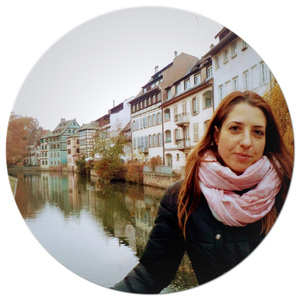
\includegraphics[height=2cm]{talia.png}
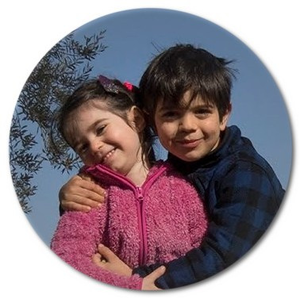
\includegraphics[height=2cm]{yoavyael.png}
\end{center}

\vfill


\end{frame}

\end{document}